The core piece of infrastructure we need to realize our approach is a
mechanism to replay execution logs. Building such a replay mechanism comes
with many challenges; unlike the example applications described
by the original delta debugging paper~\cite{Zeller:1999:YMP:318773.318946}, the system we are troubleshooting is not a
single program--it encompasses all the nodes and links of a distributed system,
including controllers, switches, and end-hosts. The asynchrony of distributed
systems makes it difficult to reliably replay orderings of
events without great care.

Our approach is to simulate the control-plane
behavior of network devices (with support for minimal data-plane behavior) on
a single machine. We then run the control software on
top of this simulator and connect the software switches to the controllers as if they were true
network devices, such that the controllers believe they are configuring a true
network. This setup allows the simulator to interpose on all communication
channels and delay, drop, or reorder
messages as needed. The overall
simulation architecture is depicted in
Figure~\ref{fig:architecture}.

\begin{figure}[t]
    %\hspace{-10pt}
    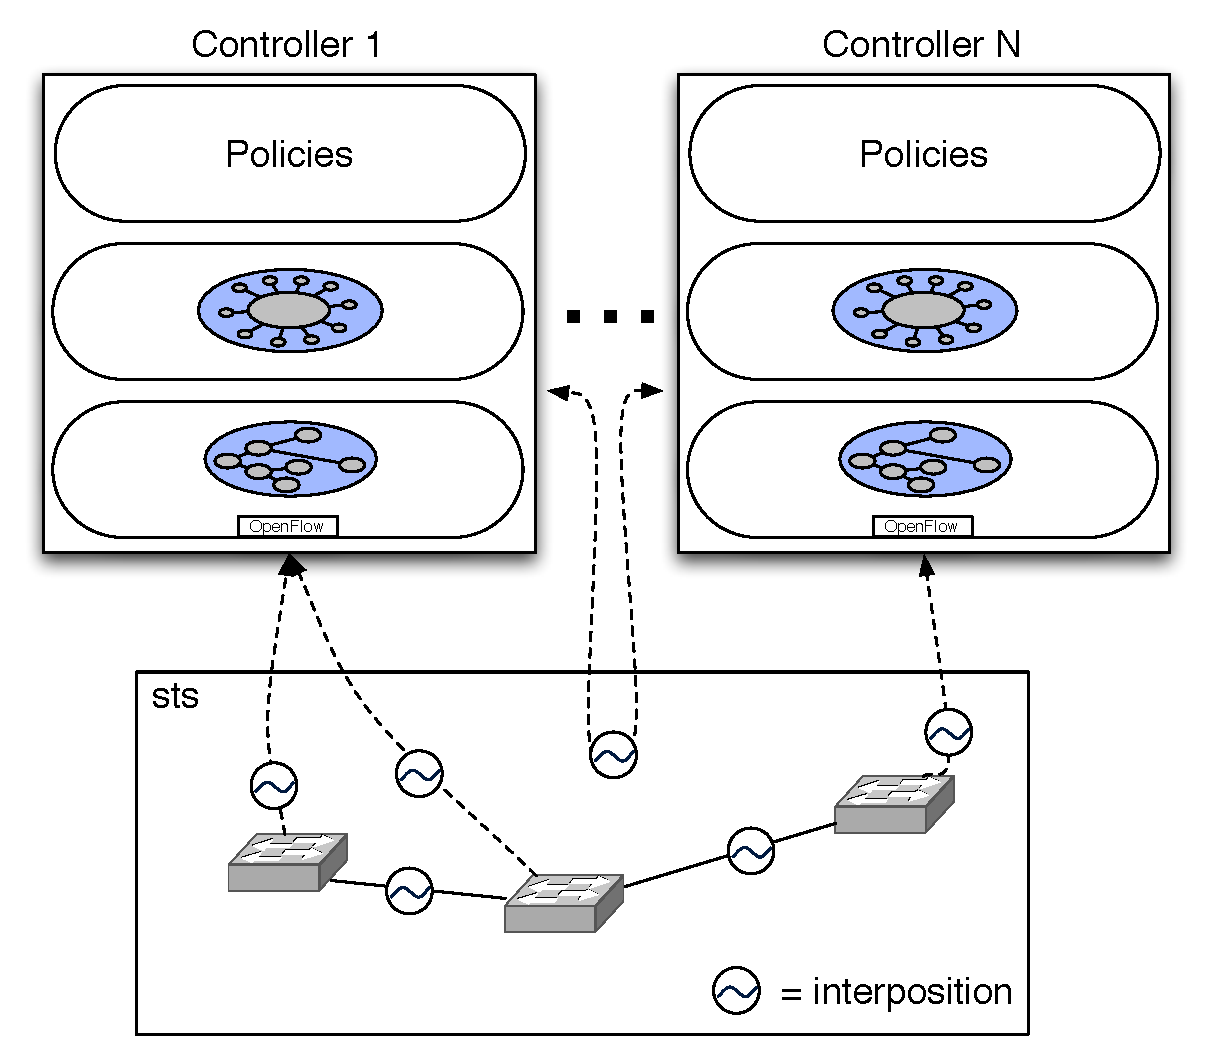
\includegraphics[width=3.25in]{../diagrams/architecture/Debugger_Architecture.pdf}
    \caption[]{\label{fig:architecture} Simulation infrastructure. We simulate
    network devices in software, and interpose on all communication
    channels.}
\end{figure}

We begin by using our simulator to perform testing on controllers to find
bugs. Our most common use case involves generating randomly chosen input
sequences~\cite{Miller:1990:ESR:96267.96279}, feeding them to controller(s),
and monitoring
invariants~\cite{hsa} at chosen intervals.
We also run the simulator interactively
so that we can examine the state of any part of the simulated network,
observe and manipulate messages, and follow our
intuition to induce orderings that we believe may trigger bugs.
Either way, controlling the inputs from a single location
allows the simulator to easily record a global, causally-consistent
event ordering.

After discovering an invariant violation of interest, the simulator replays
the logged sequence of inputs (such as link failures, controller crashes, host migrations,
or policy changes). For example, the simulator replays link failures
by disconnecting the edge in the simulated network, and sending a
port status message from the adjacent switches to their parent controller(s).

\eat{ % Maybe add this back in? This is relatively important
The input subsequences chosen by delta debugging are not always valid. For
example, it is not sensible to replay a recovery event without a
preceding failure event; nor is it sensible to replay a host migration
event without modifying its starting position when a preceding host
migration event has been pruned. The simulator checks
validity before replaying a given subsequence to account for this
possibility.\footnote{Handling invalid inputs is crucial for
ensuring that the delta debugging algorithm we employ~\cite{Zeller:1999:YMP:318773.318946}
is guaranteed to find a minimal causal sequence, since it assumes that no unresolved
test outcomes occur. Zeller wrote a follow-on
paper~\cite{Zeller:2002:SIF:506201.506206} that removes the need for this assumption,
but incurs an additional factor of $N$ in complexity in doing so.}
Currently our simulator accounts for validity of all network state change
events (shown in Table \ref{tab:inputs}), but does not support policy changes,
which have more complex semantics.
}

\colin{Cut? 15,000 LOC systems don't jive so well with HotNet's agenda}
\projectname~(\projectmeaning) is our realization of this simulator.
\projectname~is implemented in roughly 15,000 lines of Python in
addition to the Hassel network invariant checking library~\cite{hsa}. We have
made the code
for \projectname~publicly available\footnote{Omitted to preserve anonymity.} and have discussed its internal use with several commercial companies.

\subsection{Mitigating Non-Determinism}

We designed \projectname~to be as resilient to non-determinism as is
practically feasible, while avoiding modifications to control software whenever possible.
Routing the {\tt gettimeofday()} syscall
through \projectname~makes replay more resilient to alterations in execution
speeds.\footnote{When the pruned trace differs from the original, we make a
best-effort guess at what the return values of these calls should be. For example,
if the altered execution invokes {\tt gettimeofday()} more times than we recorded
in the initial run, we interpolate the time values of neighboring events}
When sending data over multiple sockets, the operating system exhibits
non-determinism in the order it schedules the socket I/O operations.
\projectname~optionally ensures a deterministic order of messages
by multiplexing all sockets in the controller process
onto a single true socket. \projectname~currently overrides socket functionality within the control
software itself.\footnote{Only supported for POX at the moment.}
%In the future we plan to implement deterministic message ordering without code modifications by
%loading a shim layer on top of
%libc (similar to liblog~\cite{Geels:2006:RDD:1267359.1267386}).

\projectname~needs visibility into the control software's internal state
changes to reliably reproduce the system execution. We achieve this by
making a
small change to the control software's logging library\footnote{Only supported
for POX and Floodlight at the moment.}: whenever a control process executes a log
statement, we notify \projectname~that a new state transition
is about to occur, and optionally block the process. \projectname~then sends
an acknowledgment to unblock the controller after logging the state change. If blocking was enabled
during recording, we force the control software to block at internal state
transition points again during replay
until \projectname~gives explicit acknowledgment.

\subsection{Coping with Non-Determinism}

Our current implementation does not account for other sources of non-determinism,
such as random number generators, asynchronous signals,
or interruptable instructions (\eg~x86's block memory
instructions~\cite{Dunlap:2002:REI:844128.844148}). And even if these sources were
eliminated, it would not be possible to achieve perfectly deterministic
replay in all cases without full visibility into internal events--a daunting
instrumentation task.

Fortunately we can cope with cases of excessive non-determinism by replaying each subsequence chosen
by delta debugging multiple times. If the non-determinism of observing the bug
is an independent and identically distributed random variable (which is an optimistic assumption) with some underlying probability $p$, then $n$
replays will observe the bug with probability $1-(1-p)^{n}$. The exponential
works strongly in our favor; for example, even if the original bug is
triggered in only 20\% of replays, the probability that we will not trigger
it during an intermediate replay is approximately
1\% if we replay 20 times per subsequence.

\subsection{Limitations}
\label{subsec:non_goals}

Having detailed the specifics of our approach we now
clarify the scope of our technique's use.

\noindent{\bf Partial Visibility.} Our event scheduling algorithm assumes that
it has visibility into the occurrence of all relevant internal events. This
may involve substantial instrumentation effort beyond
pre-existing log statements.

\noindent{\bf Non-determinism Within Individual Controllers.} Our techique is not designed to reproduce bugs
involving non-determinism within a single controller (\eg~race-conditions between threads);
we focus on coarser granularity errors (\eg~incorrect failover logic).
%The upshot of
%this is that our technique is not able to minimize all possible failures.
%Nonetheless, our worst case is that the developer ends up with what they started:
%an unpruned log.

\eat{That said, if the developer is willing to instrument their system to
provide finer granularity log messages (\cf~\cite{Geels:2006:RDD:1267359.1267386}),
our approach readily supports deterministic replay.}

\eat{
\noindent{\bf Troubleshooting vs.\ Debugging.} Our technique is a troubleshooting tool, not a debugger;
by this we mean that our approach helps identify and localize inputs that
trigger erroneous behavior, but it does not directly identify which
line(s) of code cause the error.}

\noindent{\bf Bugs Outside the Control Software.} Our goal is not to find the root
cause of individual component failures in the system (\eg~misbehaving routers,
link failures). Instead, we focus on
how the distributed system as a whole reacts to the occurrence of such inputs.
%If there is a bug in your switch, you will need to contact your hardware vendor;
%if you have a bug in your policy specification, you will need to take a closer look at what you specified.

%\noindent{\bf Globally vs.\ Locally Minimal Input Sequences.}
%Our approach is not guaranteed to find the globally minimal
%causal sequence from an input trace, since this enumerating the powerset of
%$E_L$ in the worst case (a $O(2^n)$ operation).
%The delta debugging algorithm we employ does provably find a
%locally minimal causal sequence~\cite{Zeller:1999:YMP:318773.318946},
%meaning that if any input from the sequence is pruned, no invariant violation
%occurs. \colin{Need to mention monotonicity, consistency, unambiguity here}

\noindent{\bf Correctness vs.\ Performance.}
We are primarily focused on correctness bugs, not performance bugs.

\noindent{\bf Complexity.}
The overall runtime of our technique is
$O(nlog\,n)$ in the number of replayed inputs in the best case,
and $O(n^2)$ in the worst case.
%We are currently exploring techniques such as
%parallelization and snapshotting for improving the overall runtime.

\noindent{\bf Bugs Found Through Fuzzing.}
We generate bug traces primarily through fuzz testing, not from real bugs
found in operation. There is a substantial practical hurdle in instrumenting operational systems to produce logs that can be injected into our system, and we have not addressed those issues yet.
%In practice some bugs
%found through fuzzing will not be considered worthwhile to investigate.

\noindent{\bf Scaling.}
Our discussions with companies with large SDN deployments suggest that scaling to the size of the large logs they collect will be a substantial challenge.  On the other hand, the fact that these logs are so large makes the need for finding MCSes even more acute.

\eat{
\noindent{\bf Proactive vs.\ Reactive Configuration.} We focus primarily on
\emph{proactive} configuration, where controllers react to policy and topology changes, but
not necessarily individual packets or flows events in the
dataplane.\footnote{Production controllers typically adopt this model for
performance reasons.}
The main challenge in extending our approach to reactive controllers is
achieving efficient simulation of dataplane traffic.
\andi{Could cut this. We actually find reactive bugs}
}

